\documentclass{article}
\usepackage[utf8]{inputenc}


\title{Resumen de  Vídeo}
\author{Bryan Padilla}
\date{21/01/2020}

\usepackage{natbib}
\usepackage{graphicx}

\begin{document}

\maketitle

\section{¿Qué es programar?}
\large
La Programación es la acción y efecto de programar, se refiere a idear y ordenar las acciones a un Sistema  
Especificar	la	estructura y	el	comportamiento de	un	programa,	así	como	probar que	el	programa	realiza	su	tarea	adecuadamente y	con	un	rendimiento aceptable.\\
Programar es codificar instrucciones para realizar una actividad, en un lenguaje de programación con la finalidad de que sean ejecutadas por la computadora para solucionar un problema.\

\begin{figure}[h!]
\centering

\includegraphics[scale=0.9]{lenguajes.jpg}\\[2cm]
\end{figure}

\section{¿Cómo se programa?}
\large
En este punto lo mejor que puedes hacer es realiza una comparativa e ir bajando el nivel de detalle desde el habla humana hasta el lenguaje del ordenador.\\
El hecho de comunicarse es una de las primeras acciones que llevó a cabo el ser humano al vivir en comunidad. Tenían que comunicarse los unos con los otros para poder llevar a cabo todos juntos acciones tan básicas como cazar para comer.

\begin{figure}[h!]
\centering

\includegraphics[scale=0.9]{hablar.png}
\end{figure}

\begin{center}

   \large La comunicación de las personas con los ordenadores llegamos al mismo punto, la persona tiene que decirle al ordenador qué es lo que tiene que hacer y cómo lo tiene que hacer. Para ello existen multitud de lenguajes programación.
\end{center}

\begin{figure}[h!]
\centering

\includegraphics[scale=0.26]{eje.jpg}\\[1cm]
\end{figure}
 
\section{¿Para qué sirve programar?} 
\large
 Programar te sirve para comunicarte con cualquier computadora, smartphone, tablet se vuelve indispensable para la tecnología, a la innovación o incluso a trabajar en cualquiera de las ramas a las que te dediques y desees construir tu propio sitio web. 
 
\begin{figure}[h!]
\centering
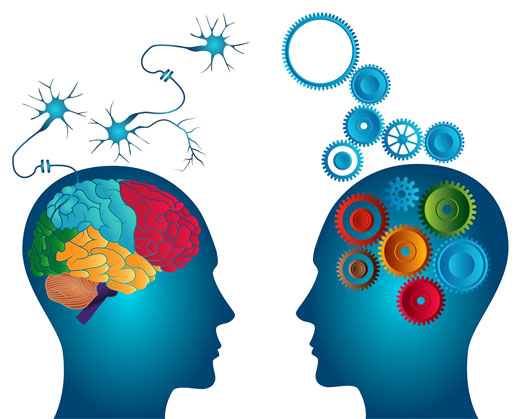
\includegraphics[scale=0.5]{3925.jpg}
\end{figure}

\begin{figure}[h!]
\centering
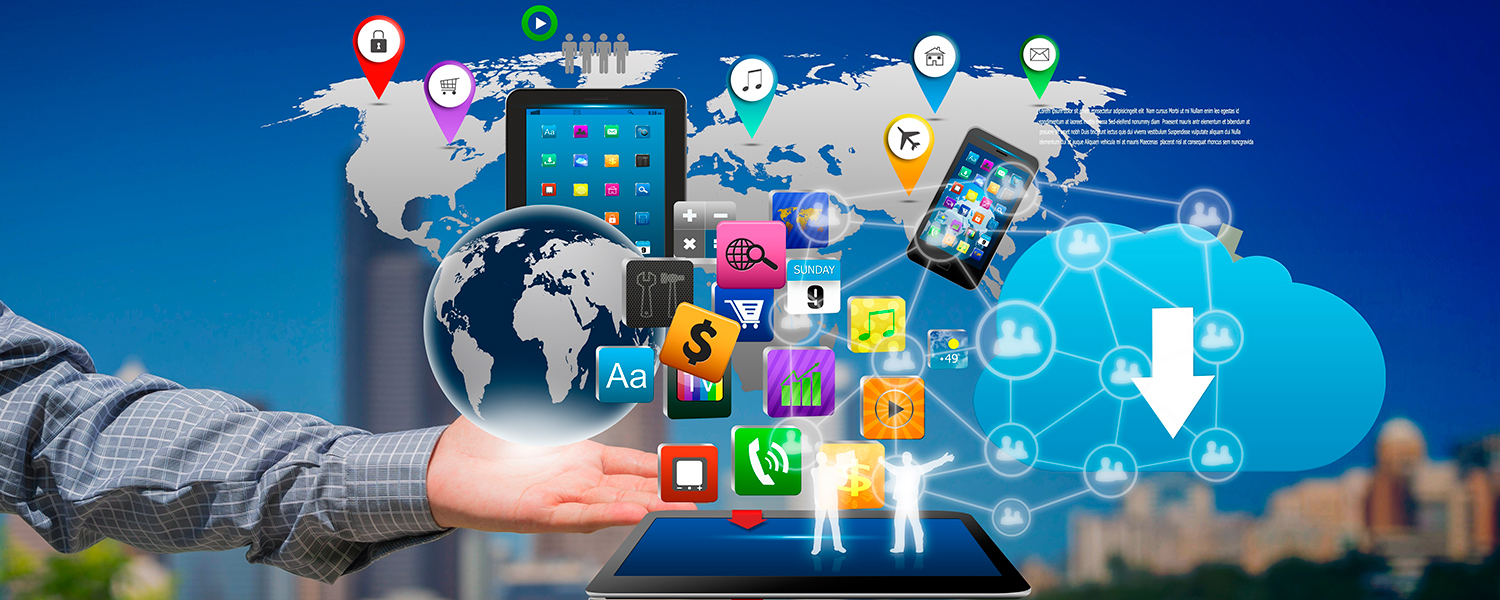
\includegraphics[scale=0.23]{Android-1.jpg}
\end{figure}






\end{document}
